% !TeX program = pdflatex
\documentclass[aspectratio=169,utf8,t]{beamer}

% Idioma e Codificacao
\usepackage[brazilian]{babel}
\usepackage{booktabs}
\usepackage{array}
\usepackage{listings}
\usepackage{amsmath}
\usepackage{amssymb}
\usepackage{graphicx}
\usepackage{tikz}
\usetikzlibrary{shapes,arrows,positioning,calc,shapes.multipart}

% Carrega o Tema Modelo dos Scouts (Widescreen 16:9, Nunito Sans)
\usetheme{scouts}

% Definicao de linguagem JavaScript/JSON/MongoSH para o listings
\lstdefinelanguage{mongosh}{
  keywords={use, show, db, dbs, collections, insertOne, insertMany, find, findOne, updateOne, updateMany, deleteOne, deleteMany, bulkWrite, createIndex, dropIndex, getIndexes, listIndexes, explain, ObjectId, ISODate, NumberDecimal, Decimal128, true, false, null},
  sensitive=true,
  comment=[l]{//},
  morecomment=[s]{/*}{*/},
  morestring=[b]",
  morestring=[b]'
}

% Configuracao para Codigo-Fonte (MongoSH / Python / JSON)
\lstset{
    basicstyle=\fontsize{5.2pt}{6.3pt}\selectfont\ttfamily,
    keywordstyle=\bfseries\color{ScoutNavy},
    stringstyle=\color{ScoutGreen},
    commentstyle=\itshape\color{gray},
    backgroundcolor=\color{black!3},
    frame=single,
    rulecolor=\color{black!15},
    breaklines=true,
    breakatwhitespace=true,
    showstringspaces=false,
    tabsize=2,
    aboveskip=2pt,
    belowskip=1pt,
    literate={á}{{\'a}}1 {ã}{{\~a}}1 {â}{{\^a}}1 {à}{{\`a}}1
             {é}{{\'e}}1 {ê}{{\^e}}1 {í}{{\'i}}1 {ó}{{\'o}}1
             {õ}{{\~o}}1 {ô}{{\^o}}1 {ú}{{\'u}}1 {ç}{{\c{c}}}1
             {Á}{{\'A}}1 {Ã}{{\~A}}1 {É}{{\'E}}1 {Í}{{\'I}}1
             {Ó}{{\'O}}1 {Õ}{{\~O}}1 {Ú}{{\'U}}1 {Ç}{{\c{C}}}1
}

% Metadados Institucionais
\author{Prof. Me. Reginaldo Fernandes}
\institute{Instituto Federal do Ceará -- Campus Tauá \\ Tecnologia em Análise e Desenvolvimento de Sistemas}
\title{Bancos de Dados Não-Relacionais}
\subtitle{Aula 07: CRUD Avançado, Atualizações Atômicas e Indexação de Alta Performance no MongoDB}
\date{03 de Novembro de 2026}

\begin{document}

% ------------------------------------------------------------------------------
% Capa da Apresentacao
% ------------------------------------------------------------------------------
\changecolours[inverse]{ScoutGreen}
\frame[plain]{\titlepage}

% ------------------------------------------------------------------------------
% Sumario Executivo da Aula
% ------------------------------------------------------------------------------
\changecolours{ScoutGreen}
\begin{frame}{Agenda do Encontro}
  \vspace{0.3cm}
  \tableofcontents
\end{frame}

% ------------------------------------------------------------------------------
% Modulos da Aula
% ------------------------------------------------------------------------------
% !TeX root = main.tex
\changecolours{ScoutGreen}
\section[Gargalos de Escala e a Teoria da $B\text{-Tree}$]{Contextualização Prática: Gargalos de Escala e a Teoria da $B\text{-Tree}$}

% ------------------------------------------------------------------------------
\twocolframe[title={O Problema de Escala no E-commerce ShopGrids},leftcol=7.0cm,rightcol=7.0cm]{%
  \alert{O Cenário sob Concorrência Real}\par
  \itemseps[topsepi=0.2mm,itemsepi=0.5mm,labelsep=1.5mm,leftmargini=2.5mm]
  \scriptsize
  \begin{itemize}
    \item Na Aula 06, estruturamos os esquemas BSON do \textbf{ShopGrids} com documentos ricos.
    \item Em ambiente de desenvolvimento com 50 itens, qualquer consulta parece instantânea ($\le 1\text{ ms}$).
    \item \textbf{O Ponto de Ruptura:} Ao carregar $50.000$ produtos e $10.000$ pedidos sob tráfego concorrente, consultas sem índice geram colapso de I/O e CPU em $100\%$!
  \end{itemize}
}{%
  \alert{A Anatomia do \texttt{COLLSCAN} (\textit{Collection Scan})}\par
  \itemseps[topsepi=0.2mm,itemsepi=0.5mm,labelsep=1.5mm,leftmargini=2.5mm]
  \scriptsize
  \begin{itemize}
    \item Sem índice, o motor WiredTiger realiza uma varredura completa da coleção: \textbf{\texttt{COLLSCAN}}.
    \item \textbf{Complexidade Temporal:} $\mathcal{O}(N)$, onde $N$ é o \textbf{Tamanho da Coleção}.
    \item Cada documento BSON precisa ser carregado do disco, descompactado na memória RAM e inspecionado campo por campo.
  \end{itemize}
}

% ------------------------------------------------------------------------------
\twocolframe[title={A Estrutura de Árvore Balanceada ($B\text{-Tree}$) no WiredTiger},leftcol=7.0cm,rightcol=7.0cm]{%
  \alert{Como o MongoDB Organiza os Índices}\par
  \itemseps[topsepi=0.2mm,itemsepi=0.5mm,labelsep=1.5mm,leftmargini=2.5mm]
  \scriptsize
  \begin{itemize}
    \item Os índices no MongoDB são estruturados como \textbf{Árvores Balanceadas ($B\text{-Tree}$)}.
    \item \textbf{Nó Raiz (\textit{Root}):} Ponto de entrada com chaves ordenadas e ponteiros.
    \item \textbf{Nós Internos:} Direcionam a busca em profundidade através de bifurcações.
    \item \textbf{Nós Folha (\textit{Leaves}):} Contêm os valores indexados e o ponteiro físico direto para o documento (\textit{RecordId}).
  \end{itemize}
}{%
  \alert{Fator de Ramificação e Complexidade}\par
  \itemseps[topsepi=0.2mm,itemsepi=0.5mm,labelsep=1.5mm,leftmargini=2.5mm]
  \scriptsize
  \begin{itemize}
    \item \textbf{Fator de Ramificação ($b$):} Número de filhos por nó (típico de 50 a 200 entradas em páginas de 4 KB).
    \item \textbf{Complexidade Logarítmica:} $\mathcal{O}(\log_{b} N)$, onde $h \approx \lceil \log_{b}(N) \rceil$ denota a \textbf{Altura da Árvore}.
    \item Em vez de ler $N$ documentos, a busca descende por apenas $h$ nós balanceados na memória RAM!
  \end{itemize}
}

% ------------------------------------------------------------------------------
\twocolframe[title={Fundamentos da Árvore Balanceada ($B\text{-Tree}$)},leftcol=6.8cm,rightcol=7.4cm]{%
  \alert{O Que É uma Árvore $B\text{-Tree}$?}\par
  \itemseps[topsepi=0.1mm,itemsepi=0.3mm,labelsep=1.3mm,leftmargini=2.2mm]
  \scriptsize
  \begin{itemize}
    \item \textbf{Conceito:} Estrutura de busca auto-balanceada multidirecional ($m$-vias), projetada para operações eficientes em blocos de disco/SSD e memória RAM.
    \item \textbf{Nós com Múltiplas Chaves:} Ao contrário de árvores binárias (1 chave, 2 filhos), nós de $B\text{-Tree}$ contêm dezenas a centenas de chaves ordenadas ($k_1 < k_2 < \dots < k_n$) e direcionam múltiplos filhos ($n+1$).
    \item \textbf{Balanceamento Perfeito:} Todas as folhas residem rigorosamente na \textbf{mesma profundidade} ($h$). Divisões de nós ocorrem para cima, garantindo busca sempre em $\mathcal{O}(\log N)$.
    \item \textbf{Roteamento por Faixas:} As chaves funcionam como balizas ordenadas, saltando diretamente ao bloco alvo sem varredura sequencial.
  \end{itemize}
}{%
  \alert{Anatomia Visual e Mecanismo de Busca}\par
  \vspace{0.1cm}
  \centering
  \begin{tikzpicture}[
    scale=0.74, transform shape,
    rootnode/.style={
      rectangle split, rectangle split parts=2, rectangle split horizontal,
      draw=ScoutNavy, fill=ScoutNavy!12, line width=1pt, rounded corners=2pt,
      inner sep=3.5pt, font=\ttfamily\scriptsize\bfseries, text centered
    },
    leafnode/.style={
      rectangle split, rectangle split parts=3, rectangle split horizontal,
      draw=ScoutGreen, fill=ScoutGreen!10, line width=0.9pt, rounded corners=2pt,
      inner sep=3pt, font=\ttfamily\scriptsize\bfseries, text centered
    },
    leafnodetwo/.style={
      rectangle split, rectangle split parts=2, rectangle split horizontal,
      draw=ScoutGreen, fill=ScoutGreen!10, line width=0.9pt, rounded corners=2pt,
      inner sep=3pt, font=\ttfamily\scriptsize\bfseries, text centered
    },
    docbox/.style={
      draw=ScoutPurple, fill=ScoutPurple!8, line width=0.8pt, rounded corners=3pt,
      font=\ttfamily\tiny, inner sep=3.5pt, align=center
    },
    searchbadge/.style={
      draw=ScoutRed!90, fill=ScoutRed!6, line width=0.7pt, rounded corners=2pt,
      font=\tiny, align=left, inner sep=2.5pt
    },
    ptr/.style={->, >=stealth, line width=0.7pt, ScoutNavy!70},
    searchptr/.style={->, >=stealth, line width=1.3pt, ScoutRed}
  ]
    % Nó Raiz
    \node[rootnode] (root) at (2.4, 3.4) {20 \nodepart{two} 50};
    \node[above=1pt of root, font=\scriptsize\bfseries\color{ScoutNavy}] {Nó Raiz (\textit{Root})};

    % Badge no canto superior direito
    \node[searchbadge] (badge) at (5.7, 3.4) {%
      \textbf{\color{ScoutRed}Busca por \texttt{preco: 45}}\\[1pt]
      1. Raiz: $20 \le 45 < 50$\\[1pt]
      2. Folha: acha 45 $\to$ \textbf{RecordId}\\[1pt]
      \textbf{Apenas 2 saltos!} $\mathcal{O}(\log N)$%
    };

    % Nós Folha
    \node[leafnodetwo] (leaf1) at (0.8, 1.8) {5 \nodepart{two} 12};
    \node[leafnode] (leaf2) at (3.2, 1.8) {25 \nodepart{two} 32 \nodepart{three} \textbf{\underline{45}}};
    \node[leafnodetwo] (leaf3) at (5.6, 1.8) {60 \nodepart{two} 80};
    
    \node[below=1pt of leaf1, font=\tiny\bfseries\color{ScoutGreen!70!black}] {Folha ($< 20$)};
    \node[below=1pt of leaf3, font=\tiny\bfseries\color{ScoutGreen!70!black}] {Folha ($\ge 50$)};

    % Conexões Raiz -> Folhas
    \draw[ptr] (root.south west) -- (leaf1.north) node[midway, left=1pt, font=\tiny\color{gray}] {$< 20$};
    \draw[searchptr] (root.south) -- (leaf2.north) node[midway, right=1pt, font=\tiny\bfseries\color{ScoutRed}] {$[20, 50)$};
    \draw[ptr] (root.south east) -- (leaf3.north) node[midway, right=1pt, font=\tiny\color{gray}] {$\ge 50$};

    % Documento no disco
    \node[docbox] (doc) at (3.5, 0.45) {%
      \textbf{RecordId \#1042} (Ponteiro Físico no Disco/RAM)\\%
      \color{darkgray}\{\_id: 1042, nome: "SSD NVMe 1TB", preco: 45\}%
    };
    \draw[searchptr] (leaf2.three south) -- (doc.north -| leaf2.three south)
      node[midway, right=1pt, font=\tiny\bfseries\color{ScoutRed}] {\textit{RecordId}};
  \end{tikzpicture}
}

% ------------------------------------------------------------------------------
\begin{frame}{Exemplo Matemático Pareado: $\mathcal{O}(N)$ vs $\mathcal{O}(\log_{b} N)$}
  \vspace{-0.1cm}
  \begin{columns}[t]
    \begin{column}{0.48\textwidth}
      \alert{1. Cálculo Analítico Passo a Passo}\par
      \itemseps[topsepi=0.1mm,itemsepi=0.3mm,labelsep=1.2mm,leftmargini=2.0mm]
      \tiny
      Considere a coleção com $N = 100.000$ produtos e fator $b = 100$:
      \begin{itemize}
        \item \textbf{Sem Índice (\texttt{COLLSCAN}):}
          $$\text{Acessos}_{\text{scan}} = N = 100.000 \text{ documentos lidos}$$
        \item \textbf{Com Índice $B\text{-Tree}$ (\texttt{IXSCAN}):}
          $$h \approx \left\lceil \log_{100}(100.000) \right\rceil = \lceil 2.5 \rceil = 3$$
        \item \textbf{Acessos necessários:} Apenas \textbf{3 nós} inspecionados!
        \item \textbf{Redução de I/O:}
          $$\left( 1 - \frac{3}{100.000} \right) \times 100\% = \mathbf{99.997\%}$$
      \end{itemize}
    \end{column}
    \begin{column}{0.48\textwidth}
      \alert{2. Interpretação em Hardware}\par
      \itemseps[topsepi=0.1mm,itemsepi=0.3mm,labelsep=1.2mm,leftmargini=2.0mm]
      \tiny
      \begin{itemize}
        \item A busca sequencial exige ler megabytes de dados brutos e satura a banda do barramento PCIe/SATA.
        \item A $B\text{-Tree}$ realiza saltos diretos em blocos ordenados.
        \item Como a raiz e os nós intermediários residem no cache WiredTiger na RAM, o acesso a um registro é quase instantâneo ($\le 0.5\text{ ms}$).
      \end{itemize}
    \end{column}
  \end{columns}
\end{frame}

% ------------------------------------------------------------------------------
\begin{frame}[fragile]{Demonstração Computacional Pareada em Python}
  \vspace{0.05cm}
  \scriptsize
  Implementação em Python medindo a diferença prática entre busca linear e busca em árvore:
  \begin{lstlisting}[language=Python]
import time, bisect

N = 100_000
dados_lineares = list(range(N))
dados_ordenados = sorted(dados_lineares) # Estrutura do Indice B-Tree
alvo = 99_999 # Pior caso (elemento final)

# 1. Busca Linear O(N) -> Simulacao de COLLSCAN
t0 = time.perf_counter()
for item in dados_lineares:
    if item == alvo: break
tempo_scan = (time.perf_counter() - t0) * 1000

# 2. Busca em Arvore O(log N) -> Simulacao de IXSCAN
t0 = time.perf_counter()
pos = bisect.bisect_left(dados_ordenados, alvo)
tempo_indice = (time.perf_counter() - t0) * 1000

print(f"COLLSCAN (Linear): {tempo_scan:.4f} ms")
print(f"IXSCAN (Indice)  : {tempo_indice:.4f} ms")
# Resultado: IXSCAN eh mais de 800x mais rapido com N = 100.000!
  \end{lstlisting}
\end{frame}

% !TeX root = main.tex
\changecolours{ScoutNavy}
\section[CRUD Avançado: Filtros e Atualizações Atômicas]{CRUD Avançado: Filtros Complexos e Atualizações Atômicas}

% ------------------------------------------------------------------------------
\begin{frame}[fragile]{O Operador \texttt{\$elemMatch} e o Problema dos Falsos Positivos}
  \vspace{0.05cm}
  \begin{columns}[t]
    \begin{column}{0.48\textwidth}
      \alert{A Armadilha do Filtro Ingênuo em Arrays}\par
      \itemseps[topsepi=0.2mm,itemsepi=0.5mm,labelsep=1.5mm,leftmargini=2.5mm]
      \scriptsize
      Considere o pedido com dois itens:
      \begin{itemize}
        \item Item A: \texttt{preco = 250}, \texttt{qtd = 1}
        \item Item B: \texttt{preco = 20}, \texttt{qtd = 8}
      \end{itemize}
      Se consultarmos:
      \begin{lstlisting}[language=mongosh]
db.pedidos.find({
  "itens.preco": { $gt: 100 },
  "itens.qtd": { $gte: 5 }
})
      \end{lstlisting}
      \textbf{Resultado:} O documento é retornado! O Item A atendeu ao preço e o Item B à quantidade. O filtro avaliou itens \textbf{diferentes}!
    \end{column}
    \begin{column}{0.48\textwidth}
      \alert{A Solução Estrita com \texttt{\$elemMatch}}\par
      \scriptsize
      O operador \texttt{\$elemMatch} força o motor a exigir que \textbf{todas as condições sejam atendidas no mesmo elemento}:
      \begin{lstlisting}[language=mongosh]
db.pedidos.find({
  itens: {
    $elemMatch: {
      preco: { $gt: 100 },
      qtd: { $gte: 5 }
    }
  }
})
      \end{lstlisting}
      \textbf{Resultado:} Nenhum documento é retornado, eliminando com precisão o falso positivo!
    \end{column}
  \end{columns}
\end{frame}

% ------------------------------------------------------------------------------
\begin{frame}[fragile]{Operador \texttt{\$expr}: Comparação de Campos Internos}
  \vspace{0.05cm}
  \begin{columns}[t]
    \begin{column}{0.48\textwidth}
      \alert{Quando Usar o \texttt{\$expr}?}\par
      \itemseps[topsepi=0.2mm,itemsepi=0.5mm,labelsep=1.5mm,leftmargini=2.5mm]
      \scriptsize
      \begin{itemize}
        \item Filtros comuns comparam um campo com um valor estático (\texttt{preco > 100}).
        \item Para comparar \textbf{dois campos do mesmo documento}, usamos \texttt{\$expr}.
        \item O prefixo \texttt{\$} indica que o valor daquele campo deve ser resolvido em tempo de execução.
      \end{itemize}
    \end{column}
    \begin{column}{0.48\textwidth}
      \alert{Exemplos Práticos no E-Commerce}\par
      \begin{lstlisting}[language=mongosh]
// 1. Produtos com estoque atual abaixo do estoque minimo:
db.produtos.find({
  $expr: {
    $lt: ["$estoque.atual", "$estoque.minimo"]
  }
})

// 2. Pedidos em que total pago foi menor que o subtotal:
db.pedidos.find({
  $expr: {
    $lt: ["$pagamento.total_pago", "$pagamento.subtotal"]
  }
})
      \end{lstlisting}
    \end{column}
  \end{columns}
\end{frame}

% ------------------------------------------------------------------------------
\begin{frame}[fragile]{Atualizações Atômicas Concorrentes: \texttt{\$inc}, \texttt{\$min} e \texttt{\$max}}
  \vspace{0.05cm}
  \begin{columns}[t]
    \begin{column}{0.48\textwidth}
      \alert{Por que Evitar \texttt{\$set} para Contadores?}\par
      \itemseps[topsepi=0.2mm,itemsepi=0.5mm,labelsep=1.5mm,leftmargini=2.5mm]
      \scriptsize
      \begin{itemize}
        \item Ler o estoque para a memória da aplicação, subtrair $1$ e salvar com \texttt{\$set} causa \textbf{Condições de Corrida (\textit{Race Conditions})}.
        \item Se duas requisições concorrentes lerem estoque $10$, ambas gravarão $9$, perdendo uma venda!
        \item O operador \textbf{\texttt{\$inc}} opera diretamente no bloco de memória do WiredTiger com garantia de atomicidade.
      \end{itemize}
    \end{column}
    \begin{column}{0.48\textwidth}
      \alert{Sintaxe de Operadores Atômicos}\par
      \begin{lstlisting}[language=mongosh]
// Decrementar estoque de forma atomica:
db.produtos.updateOne(
  { sku: "SKU-INF-000101" },
  { $inc: { "estoque.atual": -2 } }
)

// Atualizar apenas se for o menor preco historico:
db.produtos.updateOne(
  { sku: "SKU-INF-000101" },
  { $min: { "historico.menor_preco": 299.90 } }
)
      \end{lstlisting}
    \end{column}
  \end{columns}
\end{frame}

% ------------------------------------------------------------------------------
\begin{frame}[fragile]{Manipulação de Arrays: \texttt{\$push}, \texttt{\$slice} e \texttt{arrayFilters}}
  \vspace{0.05cm}
  \begin{columns}[t]
    \begin{column}{0.48\textwidth}
      \alert{Manutenção do \textit{Subset Pattern}}\par
      \scriptsize
      Ao inserir avaliações ou logs, usamos \texttt{\$push} com o modificador \texttt{\$slice: -5} para manter o array limitado aos últimos 5 itens:
      \begin{lstlisting}[language=mongosh]
db.produtos.updateOne(
  { sku: "SKU-INF-000101" },
  {
    $push: {
      ultimas_avaliacoes: {
        $each: [{ nota: 5, autor: "Maria" }],
        $slice: -5 // Mantem apenas os 5 mais recentes
      }
    }
  }
)
      \end{lstlisting}
    \end{column}
    \begin{column}{0.48\textwidth}
      \alert{Modificação Seletiva com \texttt{arrayFilters}}\par
      \scriptsize
      Atualiza um subdocumento específico de um array usando o identificador \texttt{\$[alvo]}:
      \begin{lstlisting}[language=mongosh]
db.pedidos.updateOne(
  { codigo: "PED-2026-001" },
  {
    $set: {
      "itens.$[alvo].status_entrega": "SEPARADO",
      "itens.$[alvo].data": new Date()
    }
  },
  {
    arrayFilters: [ { "alvo.sku": "ITEM-A" } ]
  }
)
      \end{lstlisting}
    \end{column}
  \end{columns}
\end{frame}

% !TeX root = main.tex
\changecolours{ScoutGreen}
\section[Índices Simples, Compostos e Otimizações]{Teoria de Índices: Índices Simples, Compostos e Otimizações de Memória}

% ------------------------------------------------------------------------------
\begin{frame}[fragile]{Gestão e Anatomia de Índices no MongoDB}
  \vspace{0.05cm}
  \begin{columns}[t]
    \begin{column}{0.48\textwidth}
      \alert{Comandos Essenciais no Terminal}\par
      \itemseps[topsepi=0.2mm,itemsepi=0.5mm,labelsep=1.5mm,leftmargini=2.5mm]
      \scriptsize
      \begin{itemize}
        \item O MongoDB cria automaticamente o índice único no campo \texttt{\_id}.
        \item Todo índice adicional consome espaço em disco e memória RAM no cache do WiredTiger.
      \end{itemize}
      \begin{lstlisting}[language=mongosh]
// Listar indices existentes:
db.produtos.getIndexes()

// Remover um indice pelo nome:
db.produtos.dropIndex("idx_sku_1")
      \end{lstlisting}
    \end{column}
    \begin{column}{0.48\textwidth}
      \alert{Índice Simples (\textit{Single Field Index})}\par
      \scriptsize
      \begin{lstlisting}[language=mongosh]
db.produtos.createIndex(
  { sku: 1 },
  { unique: true, name: "idx_sku_unico" }
)
      \end{lstlisting}
      \itemseps[topsepi=0.2mm,itemsepi=0.5mm,labelsep=1.5mm,leftmargini=2.5mm]
      \begin{itemize}
        \item \textbf{Direção (1 vs -1):} Em índices simples, a direção é irrelevante para a performance, pois o motor pode percorrer a $B\text{-Tree}$ bidirecionalmente com o mesmo custo.
        \item \textbf{\texttt{unique: true}:} Garante unicidade e integridade no banco.
      \end{itemize}
    \end{column}
  \end{columns}
\end{frame}

% ------------------------------------------------------------------------------
\begin{frame}[fragile]{Índices Compostos e a Regra dos Prefixos}
  \vspace{0.05cm}
  \begin{columns}[t]
    \begin{column}{0.48\textwidth}
      \alert{O que é um Índice Composto?}\par
      \itemseps[topsepi=0.2mm,itemsepi=0.5mm,labelsep=1.5mm,leftmargini=2.5mm]
      \scriptsize
      \begin{itemize}
        \item Índice construído sobre dois ou mais campos da coleção.
        \item A ordenação é hierárquica: os nós são ordenados pelo primeiro campo; em caso de empate, pelo segundo, e assim por diante.
      \end{itemize}
      \begin{lstlisting}[language=mongosh]
db.produtos.createIndex({
  categoria: 1,
  preco: -1
})
      \end{lstlisting}
    \end{column}
    \begin{column}{0.48\textwidth}
      \alert{Correspondência de Prefixos (\textit{Index Prefixes})}\par
      \itemseps[topsepi=0.2mm,itemsepi=0.5mm,labelsep=1.5mm,leftmargini=2.5mm]
      \scriptsize
      Considere o índice composto em \texttt{\{ A: 1, B: 1, C: 1 \}}:
      \begin{itemize}
        \item \textbf{Prefixos Válidos (Acelerados):}
          \begin{itemize}\scriptsize
            \item Consulta sobre \texttt{\{ A \}}
            \item Consulta sobre \texttt{\{ A, B \}}
            \item Consulta sobre \texttt{\{ A, B, C \}}
          \end{itemize}
        \item \textbf{Consultas NÃO Aceleradas:}
          \begin{itemize}\scriptsize
            \item Consulta sobre \texttt{\{ B \}} ou \texttt{\{ C \}}
            \item Consulta sobre \texttt{\{ B, C \}} sem o campo \texttt{A}
          \end{itemize}
      \end{itemize}
    \end{column}
  \end{columns}
\end{frame}

% ------------------------------------------------------------------------------
\begin{frame}[fragile]{Otimizações de Memória RAM: Índices Parciais, Esparsos e TTL}
  \vspace{0.05cm}
  \begin{columns}[t]
    \begin{column}{0.48\textwidth}
      \alert{Índices Parciais (\textit{Partial Indexes})}\par
      \scriptsize
      Indexam apenas documentos que atendem a um filtro, economizando dezenas de megabytes no cache da RAM:
      \begin{lstlisting}[language=mongosh]
// Indexa apenas pedidos PENDENTES:
db.pedidos.createIndex(
  { cliente_id: 1, data_criacao: -1 },
  { partialFilterExpression: { status: "PENDENTE" } }
)
      \end{lstlisting}
      \itemseps[topsepi=0.2mm,itemsepi=0.5mm,labelsep=1.5mm,leftmargini=2.5mm]
      \begin{itemize}
        \item Pedidos já entregues ou cancelados não ocupam espaço na árvore balanceada!
      \end{itemize}
    \end{column}
    \begin{column}{0.48\textwidth}
      \alert{Índices TTL (\textit{Time-To-Live})}\par
      \scriptsize
      Excluem automaticamente documentos expirados do banco sem necessidade de rotinas de \textit{cron job}:
      \begin{lstlisting}[language=mongosh]
// Exclui o carrinho apos 3600 segundos:
db.carrinhos.createIndex(
  { data_expiracao: 1 },
  { expireAfterSeconds: 0 }
)
      \end{lstlisting}
      \itemseps[topsepi=0.2mm,itemsepi=0.5mm,labelsep=1.5mm,leftmargini=2.5mm]
      \begin{itemize}
        \item O motor WiredTiger roda uma thread em segundo plano a cada 60s para limpeza automática.
      \end{itemize}
    \end{column}
  \end{columns}
\end{frame}

% !TeX root = main.tex
\changecolours{ScoutNavy}
\shorthandoff{"}
\section[A Regra de Ouro ESR, Multikey e Texto]{A Regra de Ouro ESR, Índices Multikey e Busca Textual}

% ------------------------------------------------------------------------------
\begin{frame}[fragile]{A Regra de Ouro ESR (\textit{Equality, Sort, Range})}
  \vspace{0.05cm}
  \begin{columns}[t,onlytextwidth]
    \begin{column}{0.48\textwidth}
      \alert{A Ordem Mandatória dos Campos}\par
      \itemseps[topsepi=0.2mm,itemsepi=0.5mm,labelsep=1.5mm,leftmargini=2.5mm]
      \scriptsize
      Ao desenhar índices compostos que misturam filtros, ordenação e faixas, siga sempre a ordem:
      \begin{enumerate}
        \item \textbf{[E] Equality (Igualdade):} Campos filtrados por igualdade exata (\texttt{status: 'ATIVO'}).
        \item \textbf{[S] Sort (Ordenação):} Campos da cláusula \texttt{sort} (\texttt{data\_cadastro: -1}).
        \item \textbf{[R] Range (Faixa):} Campos com operadores de desigualdade (\texttt{preco: \{ \$gte: 100 \}}).
      \end{enumerate}
      \begin{lstlisting}[language=mongosh]
// Indice Composto Ideal (E-S-R):
db.produtos.createIndex({
  status: 1,         // [E]
  data_cadastro: -1, // [S]
  preco: 1           // [R]
})
      \end{lstlisting}
    \end{column}
    \begin{column}{0.48\textwidth}
      \alert{O Perigo Fatal de Quebrar a Regra ESR}\par
      \itemseps[topsepi=0.2mm,itemsepi=0.5mm,labelsep=1.5mm,leftmargini=2.5mm]
      \scriptsize
      \begin{itemize}
        \item Se colocarmos a Faixa antes do Sort (\textbf{E-R-S}): o motor varre os nós da faixa de preço, mas perde a ordenação temporal contígua da $B\text{-Tree}$!
        \item O banco é obrigado a executar uma etapa custosa de \textbf{\texttt{SORT} em memória RAM}.
        \item \textbf{Erro Fatal:} Se o volume de dados para ordenação em memória ultrapassar \textbf{100 MB}, o MongoDB aborta a consulta com erro de execução:
          \textit{Sort exceeded memory limit of 104857600 bytes}!
      \end{itemize}
    \end{column}
  \end{columns}
\end{frame}

% ------------------------------------------------------------------------------
\begin{frame}{Diagrama Arquitetural: Fluxo de Execução da Regra ESR}
  \vspace{-0.1cm}
  \begin{columns}[t,onlytextwidth]
    % Coluna 1: Regra ESR Respeitada (Streaming)
    \begin{column}{0.48\textwidth}
      \centering
      \alert{\textbf{Padrão Correto: ESR}}\par
      \vspace{1pt}
      {\scriptsize\color{ScoutNavy}\textbf{\texttt{\{ status: 1, data: -1, preco: 1 \}}}}\par
      \vspace{0.15cm}
      \begin{tikzpicture}[
        scale=0.74, transform shape,
        box/.style={rectangle, draw=ScoutNavy, fill=ScoutNavy!10, rounded corners=3pt, line width=0.8pt, font=\ttfamily\scriptsize, align=center, inner sep=4pt},
        stepE/.style={rectangle, draw=ScoutNavy!80, fill=ScoutNavy!15, rounded corners=2pt, font=\scriptsize\bfseries, inner sep=3pt, align=center},
        stepS/.style={rectangle, draw=ScoutGreen!80, fill=ScoutGreen!15, rounded corners=2pt, font=\scriptsize\bfseries, inner sep=3pt, align=center},
        stepR/.style={rectangle, draw=ScoutTeal!80, fill=ScoutTeal!15, rounded corners=2pt, font=\scriptsize\bfseries, inner sep=3pt, align=center},
        badgeOK/.style={rectangle, draw=ScoutGreen!90, fill=ScoutGreen!12, rounded corners=3pt, line width=0.8pt, font=\scriptsize\bfseries\color{ScoutGreen!80!black}, align=center, inner sep=4pt},
        flow/.style={->, >=stealth, line width=1.1pt, ScoutNavy!80}
      ]
        % Fluxo ESR
        \node[box] (query1) at (0, 3.9) {\textbf{find}(\{ status: 'ATIVO', preco: \dots \})\\\textbf{.sort}(\{ data: -1 \})};
        
        \node[stepE] (e1) at (0, 2.7) {[E] \texttt{status: 'ATIVO'}\\\tiny Salto direto ao ramo da árvore};
        \node[stepS] (s1) at (0, 1.5) {[S] \texttt{sort(data: -1)}\\\tiny Folhas contíguas já ordenadas na B-Tree};
        \node[stepR] (r1) at (0, 0.3) {[R] \texttt{preco >= 100}\\\tiny Filtro aplicado durante varredura contínua};

        \node[badgeOK] (res1) at (0, -0.9) {%
          \textbf{Pipeline Streaming (\texttt{IXSCAN} $\to$ \texttt{FETCH})}\\%
          \tiny\color{black!80}Zero memória para SORT | Primeiro doc entregue em $< 1$ ms%
        };

        \draw[flow] (query1) -- (e1);
        \draw[flow] (e1) -- (s1);
        \draw[flow] (s1) -- (r1);
        \draw[flow] (r1) -- (res1);
      \end{tikzpicture}
    \end{column}

    % Coluna 2: Regra ESR Quebrada (Bloqueio em RAM)
    \begin{column}{0.48\textwidth}
      \centering
      \alert{\textbf{Violação da Regra: E-R-S}}\par
      \vspace{1pt}
      {\scriptsize\color{ScoutRed}\textbf{\texttt{\{ status: 1, preco: 1, data: -1 \}}}}\par
      \vspace{0.15cm}
      \begin{tikzpicture}[
        scale=0.74, transform shape,
        box/.style={rectangle, draw=ScoutNavy, fill=ScoutNavy!10, rounded corners=3pt, line width=0.8pt, font=\ttfamily\scriptsize, align=center, inner sep=4pt},
        stepE/.style={rectangle, draw=ScoutNavy!80, fill=ScoutNavy!15, rounded corners=2pt, font=\scriptsize\bfseries, inner sep=3pt, align=center},
        stepR/.style={rectangle, draw=ScoutTeal!80, fill=ScoutTeal!15, rounded corners=2pt, font=\scriptsize\bfseries, inner sep=3pt, align=center},
        stepS/.style={rectangle, draw=ScoutRed!80, fill=ScoutRed!15, rounded corners=2pt, font=\scriptsize\bfseries, inner sep=3pt, align=center},
        badgeFail/.style={rectangle, draw=ScoutRed!90, fill=ScoutRed!12, rounded corners=3pt, line width=0.8pt, font=\scriptsize\bfseries\color{ScoutRed!90!black}, align=center, inner sep=4pt},
        flowRed/.style={->, >=stealth, line width=1.1pt, ScoutRed!90}
      ]
        % Fluxo Quebrado
        \node[box] (query2) at (0, 3.9) {\textbf{find}(\{ status: 'ATIVO', preco: \dots \})\\\textbf{.sort}(\{ data: -1 \})};
        
        \node[stepE] (e2) at (0, 2.7) {[E] \texttt{status: 'ATIVO'}\\\tiny Salto direto ao ramo da árvore};
        \node[stepR] (r2) at (0, 1.5) {[R] \texttt{preco >= 100}\\\tiny Varre múltiplos nós de faixa de preço};
        \node[stepS] (s2) at (0, 0.3) {[S] \texttt{data: -1} (Perdido!)\\\tiny Ordem temporal fragmentada entre nós};

        \node[badgeFail] (res2) at (0, -0.9) {%
          \textbf{Estágio Bloqueante: \texttt{SORT} em RAM}\\%
          \tiny\color{black!80}Carrega tudo na RAM | Aborta se buffer ultrapassar 100 MB!%
        };

        \draw[flowRed] (query2) -- (e2);
        \draw[flowRed] (e2) -- (r2);
        \draw[flowRed] (r2) -- (s2);
        \draw[flowRed] (s2) -- (res2);
      \end{tikzpicture}
    \end{column}
  \end{columns}
\end{frame}

% ------------------------------------------------------------------------------
\begin{frame}[fragile]{Índices Multikey (Indexando Listas e Arrays)}
  \vspace{0.05cm}
  \begin{columns}[t,onlytextwidth]
    \begin{column}{0.48\textwidth}
      \alert{Como Funciona o Índice Multikey?}\par
      \itemseps[topsepi=0.2mm,itemsepi=0.5mm,labelsep=1.5mm,leftmargini=2.5mm]
      \scriptsize
      \begin{itemize}
        \item Quando um campo armazena um array (ex: \texttt{tags: ['gamer', 'rgb', 'usb-c']}), o MongoDB cria um índice \textbf{Multikey}.
        \item O WiredTiger gera uma entrada individual na árvore para cada elemento do array.
      \end{itemize}
      \begin{lstlisting}[language=mongosh]
db.produtos.createIndex({ tags: 1 })

// Consulta acelerada pelo Multikey:
db.produtos.find({ tags: "sem fio" })
      \end{lstlisting}
    \end{column}
    \begin{column}{0.48\textwidth}
      \alert{[Atenção] A Restrição de Arrays Paralelos}\par
      \itemseps[topsepi=0.2mm,itemsepi=0.5mm,labelsep=1.5mm,leftmargini=2.5mm]
      \scriptsize
      \begin{itemize}
        \item Em um índice composto, \textbf{no máximo um dos campos indexados pode ser array}!
        \item Tentar criar índice em \texttt{\{ tags: 1, cores: 1 \}} onde ambos sejam listas causa o erro fatal:
          \textit{cannot index parallel arrays}!
        \item \textbf{Razão Matemática:} Evitar a explosão combinatória cartesiana ($M \times N$ entradas no índice por documento).
      \end{itemize}
    \end{column}
  \end{columns}
\end{frame}

% ------------------------------------------------------------------------------
\begin{frame}{Diagrama Arquitetural: Mecanismo Interno do Índice Multikey}
  \vspace{-0.1cm}
  \begin{columns}[t,onlytextwidth]
    % Coluna 1: Fan-Out de Arrays no B-Tree
    \begin{column}{0.48\textwidth}
      \centering
      \alert{\textbf{Indexação de Arrays (Desmembramento 1:$N$)}}\par
      \vspace{0.15cm}
      \begin{tikzpicture}[
        scale=0.69, transform shape,
        docbox/.style={rectangle, draw=ScoutNavy, fill=ScoutNavy!10, rounded corners=3pt, line width=0.9pt, font=\ttfamily\scriptsize, align=center, inner sep=3.5pt},
        keynode/.style={rectangle, draw=ScoutGreen!90, fill=ScoutGreen!15, rounded corners=2pt, line width=0.8pt, font=\ttfamily\scriptsize\bfseries, align=center, inner sep=3pt},
        flow/.style={->, >=stealth, line width=0.9pt, ScoutNavy!80}
      ]
        % Documento BSON
        \node[docbox] (doc) at (2.2, 3.8) {%
          \textbf{Documento BSON (Disco/RAM)}\\%
          \{\_id: 101, nome: 'Mouse',\\
          \textbf{\color{ScoutPurple}tags: ['gamer', 'rgb', 'usb-c']}\}%
        };

        % Chaves na B-Tree
        \node[keynode] (k1) at (0.4, 1.8) {'gamer'\\$\to$ Rec\#101};
        \node[keynode] (k2) at (2.2, 1.8) {'rgb'\\$\to$ Rec\#101};
        \node[keynode] (k3) at (4.0, 1.8) {'usb-c'\\$\to$ Rec\#101};

        % Conexoes Documento -> Chaves
        \draw[flow] (doc.south -| k1.north) -- (k1.north) node[midway, left, font=\tiny\color{ScoutNavy}] {Chave 1};
        \draw[flow] (doc.south) -- (k2.north) node[midway, left, font=\tiny\color{ScoutNavy}] {Chave 2};
        \draw[flow] (doc.south -| k3.north) -- (k3.north) node[midway, right, font=\tiny\color{ScoutNavy}] {Chave 3};

        % Explicacao abaixo
        \node[rectangle, draw=black!20, fill=black!3, rounded corners=3pt, font=\scriptsize, align=left, inner sep=3pt] (note) at (2.2, 0.35) {%
          \textbf{Propriedades do Multikey:}\\[1pt]
          $\bullet$ Cada elemento gera uma chave na $B\text{-Tree}$.\\[1pt]
          $\bullet$ Busca \texttt{find(\{ tags: 'rgb' \})} em $\mathcal{O}(\log N)$.\\[1pt]
          $\bullet$ Deduplicação automática na entrega.%
        };
      \end{tikzpicture}
    \end{column}

    % Coluna 2: Proibicao de Arrays Paralelos
    \begin{column}{0.48\textwidth}
      \centering
      \alert{\textbf{Por Que Arrays Paralelos São Proibidos?}}\par
      \vspace{0.15cm}
      \begin{tikzpicture}[
        scale=0.69, transform shape,
        docbox/.style={rectangle, draw=ScoutRed, fill=ScoutRed!8, rounded corners=3pt, line width=0.9pt, font=\ttfamily\scriptsize, align=center, inner sep=3.5pt},
        cartbox/.style={rectangle, draw=ScoutRed!80, fill=ScoutRed!15, rounded corners=2pt, font=\ttfamily\tiny, align=center, inner sep=2.5pt},
        badgebomb/.style={rectangle, draw=ScoutRed!90, fill=ScoutRed!12, rounded corners=3pt, line width=0.8pt, font=\scriptsize\bfseries\color{ScoutRed!90!black}, align=center, inner sep=3.5pt}
      ]
        % Documento proibido
        \node[docbox] (pdoc) at (2.0, 3.8) {%
          \textbf{Índice Composto: \texttt{\{ tags: 1, cores: 1 \}}}\\%
          tags: ['gamer', 'rgb'] ($M=2$)\\%
          cores: ['preto', 'azul', 'branco'] ($N=3$)%
        };

        % Produto cartesiano
        \node[cartbox] (c1) at (0.6, 2.2) {('gamer', 'preto')\\('gamer', 'azul')\\('gamer', 'branco')};
        \node[cartbox] (c2) at (3.4, 2.2) {('rgb', 'preto')\\('rgb', 'azul')\\('rgb', 'branco')};

        \draw[->, >=stealth, line width=0.9pt, ScoutRed] (pdoc.south west) -- (c1.north);
        \draw[->, >=stealth, line width=0.9pt, ScoutRed] (pdoc.south east) -- (c2.north);

        \node[badgebomb] (bomb) at (2.0, 0.45) {%
          \textbf{Explosão Combinatória: $M \times N = 6$ nós/doc!}\\[2pt]
          \scriptsize Com 10 tags e 10 cores $\implies \mathbf{100}$ nós por doc!\\[1pt]
          \textbf{\color{ScoutRed}Bloqueio: \textit{cannot index parallel arrays}}%
        };
      \end{tikzpicture}
    \end{column}
  \end{columns}
\end{frame}

% ------------------------------------------------------------------------------
\begin{frame}[fragile]{Índices Textuais Ponderados (\textit{Full-Text Search})}
  \vspace{0.05cm}
  \begin{columns}[t,onlytextwidth]
    \begin{column}{0.48\textwidth}
      \alert{Criação com Pesos (\textit{Weights})}\par
      \scriptsize
      Atribui prioridade matemática ao título em relação à descrição e ativa o analisador de língua portuguesa:
      \begin{lstlisting}[language=mongosh]
db.produtos.createIndex(
  {
    titulo: "text",
    tags: "text",
    descricao: "text"
  },
  {
    weights: { titulo: 10, tags: 5, descricao: 1 },
    default_language: "portuguese",
    name: "idx_busca_textual"
  }
)
      \end{lstlisting}
    \end{column}
    \begin{column}{0.48\textwidth}
      \alert{Busca e Ranqueamento por Escore}\par
      \scriptsize
      Executa a busca com radicalização (\textit{stemming}) e ordena os resultados por relevância métrica:
      \begin{lstlisting}[language=mongosh]
db.produtos.find(
  { $text: { $search: "ergonomico sem fio" } },
  {
    titulo: 1,
    preco: 1,
    score: { $meta: "textScore" },
    _id: 0
  }
).sort({ score: { $meta: "textScore" } })
      \end{lstlisting}
    \end{column}
  \end{columns}
\end{frame}

% ------------------------------------------------------------------------------
\begin{frame}{Diagrama Arquitetural: Pipeline do Índice Invertido Textual}
  \vspace{-0.15cm}
  \centering
  \begin{tikzpicture}[
    scale=0.78, transform shape,
    docbox/.style={
      rectangle, draw=ScoutNavy, fill=ScoutNavy!8, rounded corners=3pt, line width=0.8pt,
      font=\scriptsize, text width=4.35cm, align=left, inner sep=4.5pt
    },
    nlpbox/.style={
      rectangle, draw=ScoutPurple!90, fill=ScoutPurple!8, rounded corners=3pt, line width=0.8pt,
      font=\scriptsize, text width=4.35cm, align=left, inner sep=4.5pt
    },
    indexbox/.style={
      rectangle, draw=ScoutGreen!80!black, fill=ScoutGreen!8, rounded corners=3pt, line width=0.9pt,
      font=\scriptsize, text width=4.35cm, align=left, inner sep=4.5pt
    },
    querybox/.style={
      rectangle, draw=ScoutNavy!80, fill=ScoutNavy!6, rounded corners=3pt, line width=0.8pt,
      font=\scriptsize, text width=4.35cm, align=left, inner sep=4.5pt
    },
    termsbox/.style={
      rectangle, draw=ScoutPurple!80, fill=ScoutPurple!6, rounded corners=3pt, line width=0.8pt,
      font=\scriptsize, text width=4.35cm, align=left, inner sep=4.5pt
    },
    scorebox/.style={
      rectangle, draw=ScoutGreen!90!black, fill=ScoutGreen!12, rounded corners=3pt, line width=0.9pt,
      font=\scriptsize, text width=4.35cm, align=left, inner sep=4.5pt
    },
    flow/.style={->, >=stealth, line width=1.1pt, ScoutNavy!80},
    matchflow/.style={->, >=stealth, dashed, line width=1.2pt, ScoutGreen!80!black}
  ]

    % --- TRILHA 1: INGESTÃO E CONSTRUÇÃO DO ÍNDICE ---
    \node[anchor=south west, font=\tiny\bfseries\color{ScoutNavy}] at (-7.2, 3.25) {%
      \scalebox{0.95}{$\blacktriangleright$} FLUXO DE INGESTÃO (TEMPO DE ESCRITA NO BANCO):%
    };

    % 1. Documento BSON
    \node[docbox] (doc) at (-5.0, 1.85) {%
      \textbf{\color{ScoutNavy}1. Documento BSON (\#101)}\\[2.5pt]
      {\ttfamily\tiny
      \begin{tabular}{@{}ll@{}}
        \textbf{\color{ScoutNavy}titulo} \textrm{[p.\,10]:} & 'Mouse Gamer' \\
        \textbf{\color{ScoutNavy}tags} \textrm{[p.\,5]:}    & ['sem fio', 'usb'] \\
        \textbf{\color{ScoutNavy}desc} \textrm{[p.\,1]:}    & 'Mouse ergonomico'
      \end{tabular}}\\[2pt]
      {\tiny\color{black!70}* Pesos definidos no índice textual}%
    };

    % 2. Pipeline NLP
    \node[nlpbox] (nlp) at (0.0, 1.85) {%
      \textbf{\color{ScoutPurple}2. Pipeline NLP (Português)}\\[2pt]
      $\bullet$ \textbf{Tokenização:} divide em termos\\[1.5pt]
      $\bullet$ \textbf{Normalização:} minúsculas\\[1.5pt]
      $\bullet$ \textbf{Stopwords:} remove \textit{'sem', 'de'}\\[1.5pt]
      $\bullet$ \textbf{Radicais (Stemming):}\\
      \ \ \textit{'ergonomico'} $\to$ \texttt{\textbf{'ergonom'}}\\
      \ \ \textit{'mouse'} $\to$ \texttt{\textbf{'mous'}}%
    };

    % 3. Índice Invertido
    \node[indexbox] (inv) at (5.0, 1.85) {%
      \textbf{\color{ScoutGreen!80!black}3. Índice Invertido Ponderado}\\[2pt]
      {\ttfamily\tiny
      \begin{tabular}{@{}llr@{}}
        \textbf{'ergonom'} & $\to$ Doc\#101 & \textbf{[p.\,1]} \\
        \textbf{'fio'}     & $\to$ Doc\#101 & \textbf{[p.\,5]} \\
        \textbf{'gamer'}   & $\to$ Doc\#101 & \textbf{[p.\,10]} \\
        \textbf{'mous'}    & $\to$ Doc\#101 & \textbf{[p.\,11]} \\
        \textbf{'usb'}     & $\to$ Doc\#101 & \textbf{[p.\,5]}
      \end{tabular}}\\[2pt]
      {\tiny\color{black!70}* 'mous': 10 (título) + 1 (desc) = 11}%
    };

    % Setas Trilha 1
    \draw[flow] (doc.east) -- (nlp.west);
    \draw[flow] (nlp.east) -- (inv.west);

    % --- TRILHA 2: CONSULTA E RANQUEAMENTO ---
    \node[anchor=south west, font=\tiny\bfseries\color{ScoutGreen!70!black}] at (-7.2, -0.25) {%
      \scalebox{0.95}{$\blacktriangleright$} FLUXO DE CONSULTA (TEMPO DE LEITURA E RANQUEAMENTO):%
    };

    % 4. Consulta $text
    \node[querybox] (query) at (-5.0, -1.65) {%
      \textbf{\color{ScoutNavy}4. Consulta \texttt{\$text}}\\[2pt]
      {\ttfamily\tiny
      db.produtos.find(\{\\
      \ \ \$text: \{\\
      \ \ \ \ \$search: 'gamer ergonomico'\\
      \ \ \}\\
      \}).sort(\{\\
      \ \ score: \{ \$meta: 'textScore' \}\\
      \})}%
    };

    % 5. Radicais da Busca
    \node[termsbox] (terms) at (0.0, -1.65) {%
      \textbf{\color{ScoutPurple}5. Processamento da Busca}\\[2pt]
      $\bullet$ \textbf{Termos digitados:}\\
      \ \ \texttt{'gamer'}, \texttt{'ergonomico'}\\[2pt]
      $\bullet$ \textbf{Radicais gerados:}\\
      \ \ \textit{'gamer'} $\to$ \texttt{\textbf{'gamer'}}\\
      \ \ \textit{'ergonomico'} $\to$ \texttt{\textbf{'ergonom'}}\\[2pt]
      $\bullet$ \textbf{Lookup:} busca radicais no índice%
    };

    % 6. Relevância (textScore)
    \node[scorebox] (score) at (5.0, -1.65) {%
      \textbf{\color{ScoutGreen!80!black}6. Relevância (\textit{textScore})}\\[2pt]
      $\bullet$ \textbf{'gamer'}: peso 10 (título)\\[2pt]
      $\bullet$ \textbf{'ergonom'}: peso 1 (descrição)\\[3pt]
      \textbf{\color{ScoutGreen!90!black}textScore = 10 + 1 = 11.0}\\[2.5pt]
      {\scriptsize $\implies$ \textbf{Doc\#101 em 1\textsuperscript{o} lugar!}}%
    };

    % Setas Trilha 2
    \draw[flow] (query.east) -- (terms.west);
    \draw[flow] (terms.east) -- (score.west);

    % Conexão Vertical Trilha 1 -> Trilha 2
    \draw[matchflow] (inv.south) -- (score.north)
      node[midway, right=2pt, font=\tiny\bfseries\color{ScoutGreen!80!black}] {Lookup de Pesos};

  \end{tikzpicture}
\end{frame}
\shorthandon{"}

% !TeX root = main.tex
\changecolours{ScoutGreen}
\section[Diagnóstico, Covered Queries e Benchmark]{Diagnóstico com \texttt{explain()}, \textit{Covered Queries} e Benchmark}

% ------------------------------------------------------------------------------
\begin{frame}[fragile]{Auditoria de Execução: Os Modos do \texttt{explain()}}
  \vspace{0.05cm}
  \begin{columns}[t]
    \begin{column}{0.48\textwidth}
      \alert{Níveis de Auditoria do Otimizador}\par
      \itemseps[topsepi=0.2mm,itemsepi=0.5mm,labelsep=1.5mm,leftmargini=2.5mm]
      \scriptsize
      \begin{itemize}
        \item \textbf{\texttt{queryPlanner} (Padrão):} Retorna apenas o plano eleito pelo otimizador sem executar a consulta.
        \item \textbf{\texttt{executionStats} (Recomendado):} Executa a consulta e retorna métricas reais de tempo, nós examinados e documentos lidos.
        \item \textbf{\texttt{allPlansExecution}:} Executa e documenta o desempenho de todos os planos candidatos testados.
      \end{itemize}
    \end{column}
    \begin{column}{0.48\textwidth}
      \alert{Sintaxe no MongoSH / PyMongo}\par
      \begin{lstlisting}[language=mongosh]
// Executando auditoria completa:
db.produtos.find(
  { sku: "SKU-INF-000101" }
).explain("executionStats")
      \end{lstlisting}
      \itemseps[topsepi=0.2mm,itemsepi=0.5mm,labelsep=1.5mm,leftmargini=2.5mm]
      \scriptsize
      \begin{itemize}
        \item Permite aos engenheiros de dados inspecionar se a consulta está usando índice (\texttt{IXSCAN}) ou colapsando em \texttt{COLLSCAN}.
      \end{itemize}
    \end{column}
  \end{columns}
\end{frame}

% ------------------------------------------------------------------------------
\begin{frame}{Decodificando as Quatro Métricas Vitais do \texttt{executionStats}}
  \vspace{0.05cm}
  \makebox[\textwidth][c]{%
    \scriptsize
    \renewcommand{\arraystretch}{1.22}
    \begin{tabular}{p{2.8cm} p{3.2cm} p{6.0cm}}
      \toprule
      \textbf{Métrica no JSON} & \textbf{Conceito Técnico} & \textbf{Alvo de Otimização} \\
      \midrule
      \texttt{stage} & Estágio da árvore de execução. & \texttt{IXSCAN} (Sem \texttt{COLLSCAN} ou \texttt{SORT} em RAM). \\
      \texttt{totalDocsExamined} & Documentos físicos lidos do disco/cache. & Deve aproximar-se de \texttt{nReturned} (ou 0). \\
      \texttt{totalKeysExamined} & Nós da $B\text{-Tree}$ inspecionados. & Próximo a \texttt{nReturned} (afunilamento eficiente). \\
      \texttt{nReturned} & Documentos realmente devolvidos. & Volume útil solicitado pela aplicação. \\
      \texttt{executionTimeMillis} & Tempo de processamento em ms. & $\le 1\text{ ms}$ para operações pontuais. \\
      \bottomrule
    \end{tabular}%
  }
  \vspace{0.15cm}
  \centering{\scriptsize \textbf{Razão de Eficiência:} $\displaystyle \frac{\text{totalDocsExamined}}{\text{nReturned}} \quad (\text{Ideal} = 1.0; \quad \text{COLLSCAN sob } 50.000 \text{ itens} = 5.000)$.}
\end{frame}

% ------------------------------------------------------------------------------
\begin{frame}[fragile]{\textit{Covered Queries} (Consultas Cobertas): O Santo Graal da Performance}
  \vspace{0.05cm}
  \begin{columns}[t]
    \begin{column}{0.48\textwidth}
      \alert{O que é uma Consulta Coberta?}\par
      \itemseps[topsepi=0.2mm,itemsepi=0.5mm,labelsep=1.5mm,leftmargini=2.5mm]
      \scriptsize
      \begin{itemize}
        \item Todos os campos da consulta (filtro e projeção) estão presentes no próprio índice $B\text{-Tree}$.
        \item O MongoDB \textbf{NUNCA lê o documento BSON do disco}!
        \item O estágio \textbf{\texttt{FETCH}} desaparece, operando 100\% em memória RAM com \textbf{\texttt{totalDocsExamined: 0}}!
      \end{itemize}
    \end{column}
    \begin{column}{0.48\textwidth}
      \alert{Código da Consulta Coberta}\par
      \scriptsize
      \begin{lstlisting}[language=mongosh]
// 1. Criar indice cobrindo categoria, preco e sku:
db.produtos.createIndex({
  categoria: 1,
  preco: 1,
  sku: 1
})

// 2. Consulta 100% coberta:
// ATENCAO: _id: 0 eh OBRIGATORIO para evitar o FETCH!
db.produtos.find(
  { categoria: "Informática", preco: { $lte: 1500 } },
  { categoria: 1, preco: 1, sku: 1, _id: 0 }
).explain("executionStats")
      \end{lstlisting}
    \end{column}
  \end{columns}
\end{frame}

% ------------------------------------------------------------------------------
\begin{frame}{Resultados do Benchmark no Laboratório (50.000 Documentos)}
  \vspace{-0.1cm}
  \begin{figure}[htbp]
    \centering
    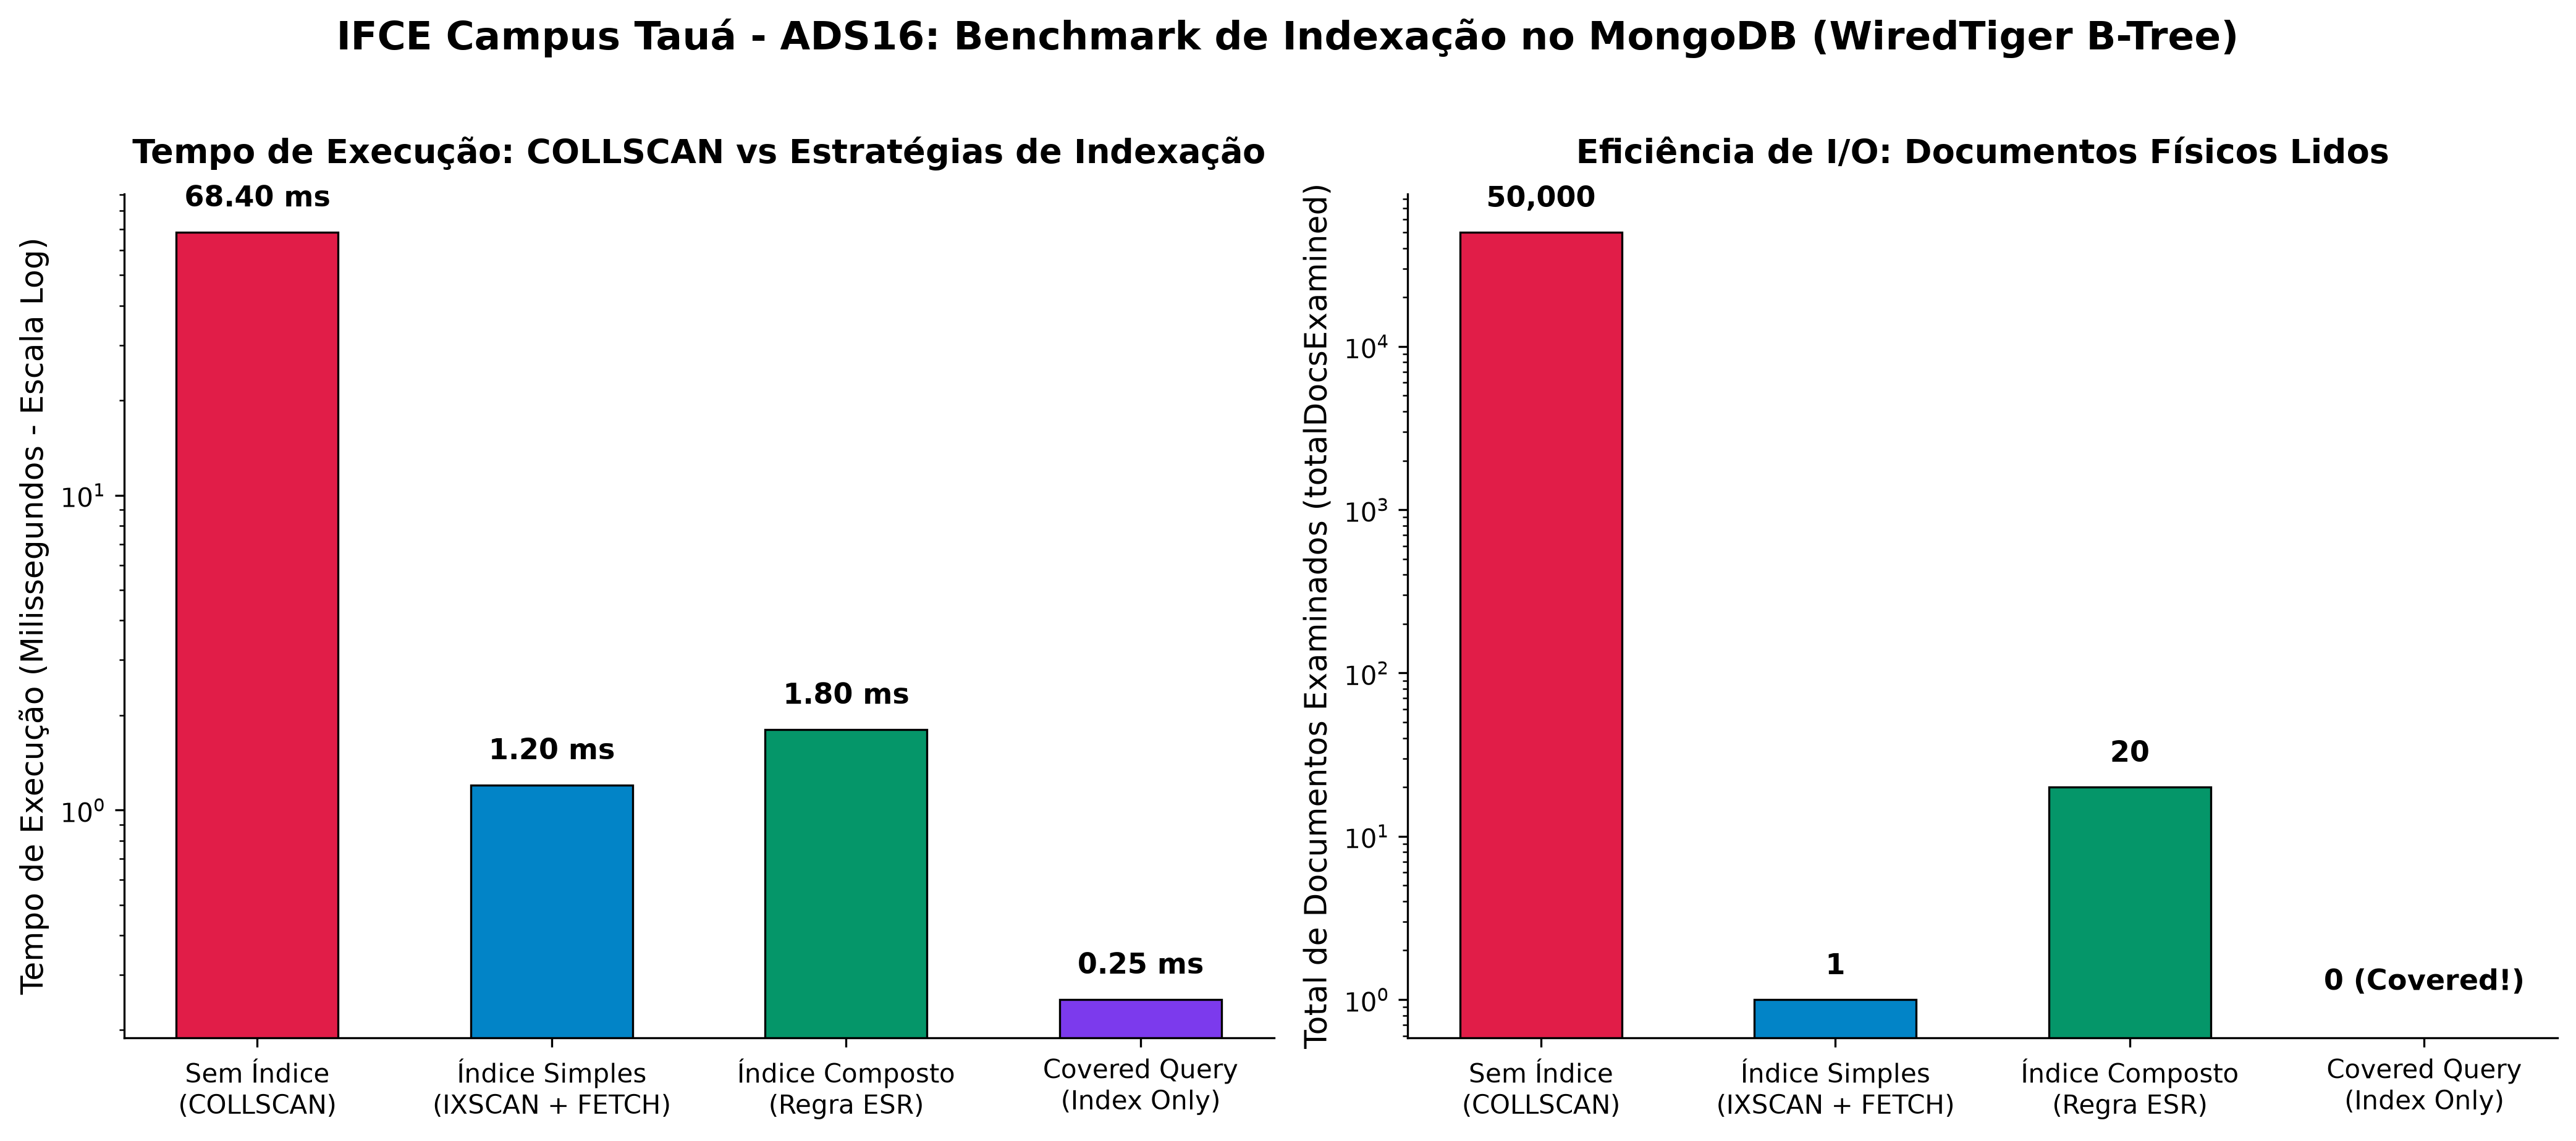
\includegraphics[width=0.90\textwidth,height=0.68\textheight,keepaspectratio]{benchmark_performance_indices.png}
  \end{figure}
  \vspace{-0.3cm}
  \centering{\tiny \textbf{Conclusão:} Adoção de índices compostos (ESR) e consultas cobertas reduz a latência em mais de $99.7\%$ e zera leituras físicas de documentos.}
\end{frame}


% ------------------------------------------------------------------------------
% Encerramento
% ------------------------------------------------------------------------------
\changecolours[inverse]{ScoutGreen}
\begin{frame}[plain]
  \vspace{2cm}
  \centering
  {\Huge \textbf{Dúvidas \& Prática em Laboratório}}\par
  \vspace{0.8cm}
  {\large IFCE Campus Tauá -- ADS16 (Modelo Orientado a Documentos)}\par
  \vspace{0.3cm}
  {\normalsize CRUD Avançado, Índices $B\text{-Tree}$, Regra ESR e Consultas Cobertas}
\end{frame}

\end{document}
